\documentclass[pdflatex,sn-mathphys-num]{sn-jnl}

\usepackage{graphicx}
\usepackage{listings}
\usepackage{xcolor}
\usepackage{booktabs}
\usepackage{float}
\usepackage{caption}
\usepackage{subcaption}
\usepackage{amsmath}
\usepackage{tcolorbox}
\usepackage{lipsum}
\usepackage{multirow}
\usepackage{mathrsfs}
\usepackage{amssymb}
\usepackage{algorithm}
\usepackage{algpseudocode}
\newtcolorbox{promptbox}{
  colback=gray!15,
  colframe=black,
  boxrule=0.5pt,
  arc=0pt,
  left=3pt, right=3pt,
  top=3pt, bottom=3pt,
  fontupper=\small
}

\begin{document}

\title{Data Shapley}

\author*[1]{\fnm{Carlo} \sur{Falchi}}\email{cfalchi@gmail.com}

\affil[1]{\orgdiv{Department of Computer Science}, \orgname{University of Milan}, \country{Italy}}

\abstract{
    Data quality is a critical factor in the performance of supervised learning algorithms. 
In this work, we apply the Data Shapley framework to assess the value of individual 
training data points by treating each datum as a player in a cooperative game. 
We estimate Data Shapley values using the Truncated Monte Carlo Shapley (TMC-Shapley) 
algorithm and evaluate the framework on two datasets: a real-world bank marketing 
dataset and a synthetic dataset generated from a Gaussian distribution, using logistic 
regression as the learning algorithm. Our experiments demonstrate that sequentially 
removing the lowest-value data points improves model performance significantly faster 
than random removal, while discarding high-value points causes rapid performance 
degradation. Furthermore, robustness experiments confirm that the framework 
effectively identifies mislabeled data points, successfully detecting 60\% of corrupted 
labels by inspecting less than 20\% of the training set ranked by Shapley value, 
outperforming random inspection by a large margin.
}

\maketitle
\section{Introduction}
The goal of the project is to assess the quality of data points used for training a model based on the Shapley values, which, in cooperative game theory, is a method for fairly distributing the total gains or costs among a group of players who have collaborated. In this case, the connection with machine learning and learning algorithms considers every data point as a player of the team. 
To achieve this evaluation, we will base our discussion on the Data Shapley framework  \cite{ghorbani2019data}, using two different datasets, a real dataset about a bank marketing campaign and a synthetic dataset generated by a Gaussian distribution. The Logistic regression is used as the learning algorithm. 
We will start by explaining how we estimate the quality of the data points, giving them a rank, and applying different fractional remove strategies to see how the performance of our predictor changes.
Further analysis will be considered, injecting noise to data points to evaluate the robustness of the method.

\section{Data Shapley}

The Data shapley framework tries to answer the question of what is an equitable measure of the value of a training datum $(x_i,y_i)$ to the supervised learning algorithm $\mathscr{A}$ with respect to the performance metric $V$

\begin{itemize}
    \item \textbf{Training set} Let $D = \{(x_i,y_i)\}^n_1$ be our fixed training set from $n$ different data sources where $(x_i, y_i)$ is the i'th source and every source could be a single input-output pair or set of pairs. $y_i$ could be Real for regression or $Categorical$ for classification.
    \item \textbf{Learning Algorithm} $\mathscr{A}$ takes the training dataset $D$ and returns a predictor
    \item \textbf{Performance Score} $V(S,\mathscr{A})$ to denote the performance score of the predictor trained on data $S$ using the learning algorithm $\mathscr{A}$
\end{itemize}

For every data point $(x_i,y_i) \in D$ (for simplicity $i$ is the same of $(x_i,y_i)$) we compute the \textbf{data value} and denote it as $\phi_i(D,\mathscr{A},V) \in \mathbb{R}$
where the following equitable valuation conditions \cite{ghorbani2019data} should be satisfied:

\begin{enumerate}
    \item \textbf{Zero Value Datapoints}: if $(x_i,y_i)$ $\forall S \subseteq D -\{i\}$, $V(S) = V(S \cup \{i\})$ then $\phi_i = 0$
    \item \textbf{Same Value for different Datapoints}: if for $i$ and $j$ data and $\forall S \subseteq D - \{i,j\}$, $V(S \cup \{i\}) = V(S \cup \{j\})$ then $\phi_i = \phi_j$
    \item \textbf{Overall performance score is the sum of separate performance scores}: $\phi_i (V + W) = \phi_i(V) + \phi_i(W)$. Given $V_k = -l_k$ where $l_k$ is the loss of the predictor in the $k$-th test point and $\phi_i(V_k)$ quantify the value of $i$-th source for predicting the $k$-th test point. We expect that with $V = V_1 + V_2$ then $\phi_i({V}) = \phi_i({V_1}) + \phi_i({V_2})$
\end{enumerate}

Any data valuation that satisfies the properties 1-3 above must have the form:
\begin{equation} \label{eq:shapley}
\displaystyle \phi_i = C \sum_{S \subseteq D - \{i\}} \frac{V(S \cup \{i\}) - V(S)}{\binom{n-1}{|S|}}
\end{equation}
where the sum is over all subsets of $D$ not containing $i$ and $C$ is an arbitrary constant. 
$\phi_i$ is the Data Shapley value of source $i$.

Each source in the train data is a player, and the players work together through the learning algorithm $\mathscr{A}$ to achieve a prediction score $v(D) = V (D, \mathscr{A})$ where $v:2^{[n]} \to \mathbb{R}$.
However computing data Shapley value requires an exponentially large number of computations
with respect to the number of train data sources. For this reason the "Truncated Monte Carlo Shapley" (TMC-Shapley) is developed, where a random permutation of sources in the train data is considered.
\section{Truncated Monte Carlo Shapley}

Calculating the exact Shapley value for each data point using the formula shown in \ref{eq:shapley} is not tractable in practice because it requires computing all marginal contributions 
for every possible permutation. An approximation called the Monte Carlo method helps to estimate these values and reduce computational costs. It samples random permutations of data points 
and calculates the marginal contribution for every data point within them; thus, the final Shapley value is the average of all the calculated marginal contributions across these different 
random permutations.

$$\phi_i = \mathbb{E}_{\pi \sim \Pi} [V(S_{\pi}^i \cup \{i\}) - V(S_{\pi}^i)]$$ 

where $S^i_{\pi}$ is the set of data points coming before datum $i$ in permutation $\pi$.

Furthermore, the algorithm \ref{alg:tmc_shapley} calculates the variation of every marginal contribution to monitor its fluctuations.
Given the intrinsic noise of the test set, and the fact that this variation reduces as the train dataset grows,
it is sufficient to calculate it only until these changes become smaller than the intrinsic error of the test set itself.
Thus the algorithm truncates the calculation of marginal contributions whenever $V(S)$ is within the performance tolerance of $V(D)$ and
sets the marginal contribution to be zero for the rest of the data points in the respective permutation.

% TODO: modify the algorith adding the convergence criterion
\begin{algorithm}
\caption{Truncated Monte Carlo Shapley}
\label{alg:tmc_shapley}
\begin{algorithmic}
\State \textbf{Input:} Train data $D = \{1,\dots,n\}$, learning algorithm $\mathcal{A}$, performance score $V$
\State \textbf{Output:} Shapley value of training points: $\phi_1,\dots,\phi_n$
\State Initialize $\phi_i = 0$ for $i = 1,\dots,n$ and $t = 0$
\While{Convergence criteria not met}
    \State $t \gets t + 1$
    \State $\pi^t$: Random permutation of train data points
    \State $v_0^t \gets V(\emptyset, \mathcal{A})$
    \For{$j \in \{1,\dots,n\}$}
        \If{$|V(D) - v_{j-1}^t| < \text{Performance Tolerance}$}
            \State $v_j^t = v_{j-1}^t$
        \Else
            \State $v_j^t \gets V(\{\pi^t[1],\dots,\pi^t[j]\}, \mathcal{A})$
        \EndIf
        \State $\phi_{\pi^t[j]} \gets \frac{t-1}{t}\phi_{\pi^{t-1}[j]} + \frac{1}{t}(v_j^t - v_{j-1}^t)$
    \EndFor
\EndWhile
\end{algorithmic}
\end{algorithm}

Figure \ref{fig:convergence} displays the algorithm's convergence for 10 random individual data points (left) and the evolution of the standard deviation of the mean over the final five iterations as the number of steps increases (right); the convergence criterion is met after 151 iterations in the 'Bank Campaign Dataset' experiment.
\begin{figure}[ht]
    \centering
    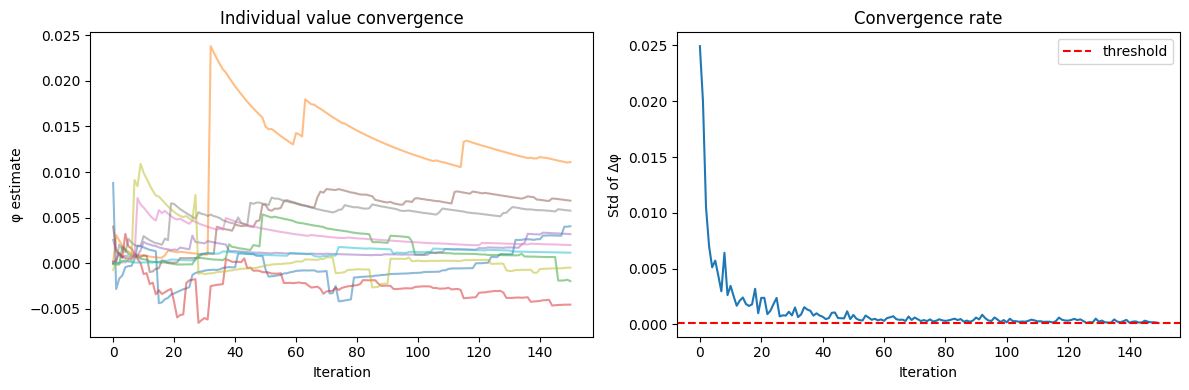
\includegraphics[width=0.9\textwidth]{charts/convergence.png}
    \caption{(Left) Convergence of 10 data papoints, (Right) Standard Deviation of the mean over the last 5 iterations}
     \label{fig:convergence}
\end{figure}
\section{Data Set}

For the evaluation of the the quality of the data points we use two different datasets, a real one, which is based on a Bank Marketing campaign \cite{moro2014bank} and a Synthetic dataset generated by a Gaussian distribution.
\subsection{Bank Campaign Data Set}
The data is related with direct marketing campaigns (phone calls) of a Portuguese banking institution. The classification goal is to predict if the client will subscribe to a term deposit.
There are 20 features (age, job, education, balance, loan etc..) in various format types: integer, binary, categorical and date, so a preprocessing is needed to convert non numerical features.
The dataset contains 4119 elements which are unbalanced, we sampled the negative customers to create a new balanced dataset (421 yes customers, 421 no customers),
then we split it in two parts,20\% is used as a testing set and 80\% is used as a training set.

\subsection{Synthetic Data Generation}

The generated synthetic dataset is designed specifically to test Data Valuation algorithms. It creates a "ground truth" where we know exactly which data points are "good" and which are noisy, to see if their model can correctly identify the low-value samples.

The process begins by generating feature vectors from a Gaussian distribution. Labels are then assigned using a Logistic Regression model, where only the first five features carry predictive weight and the rest are uninformative noise. After creating these "clean" labels, the script intentionally injects label noise by flipping a percentage of the training labels.

\section{Logistic Regression as Learning Algorithm}

For this experiment we want to output the probability that a certain data point belongs to a class (yes or no), this corresponds to the problem of learning the function $\eta(x) = P(Y = 1 \mid X = x)$ in a binary classification problem.
To do that we use the logistic regression predictor, which applies the logistic (sigmoid) function:
$$\sigma(z) = \frac{1}{1 + e^{-z}} \in (0, 1)$$
where $z = g(x)$ in our case is a linear model $\vec{w}^Tx$ and the relative loss used to train the model is the logistic loss $\ell(y, z) = \log_{2} (1 + e^{-y z})$


Then we apply the Gradient Descent to train the predictor as follows: 
$$\mathbf{w}_{t+1} = \mathbf{w}_t + \frac{\eta}{N \ln 2} \sum_{i=1}^{N} y_i \mathbf{x}_i \sigma(-y_i (\mathbf{w}^T\mathbf{x}_i))$$




\section{Evaluation}

The accuracy of the logistic regression predictor is calculated as: $\frac{1}{N} \sum_{i=1}^{N} \mathbb{I}(\hat{y}_i = y_i)$
The baseline accuracy of the predictors on the respective datasets are: 
\begin{itemize}
    \item Bank dataset: Accuracy $86.19\%$
    \item Synthetic dataset ($35\%$ of noisy labels): $88.50\%$
\end{itemize}

To evaluate the datapoints we ran the algorithm \ref{alg:tmc_shapley} using the logistic regression as learning algorithm on both the datasets mentioned before and we gave a rank to every value (Table \ref{tab:rank_bank} and \ref{tab:rank_synth}).

\begin{figure}[ht]
    \centering
    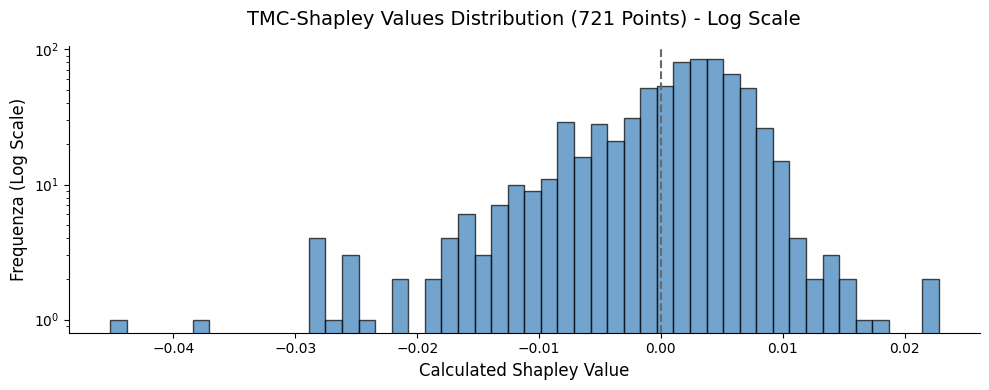
\includegraphics[width=0.9\textwidth]{charts/shapley_distribution_bank.png}
    \caption{Data shapley values of the bank marketing dataset}
     \label{fig:shapley_distribution_bank}
\end{figure}

\begin{figure}[ht]
    \centering
    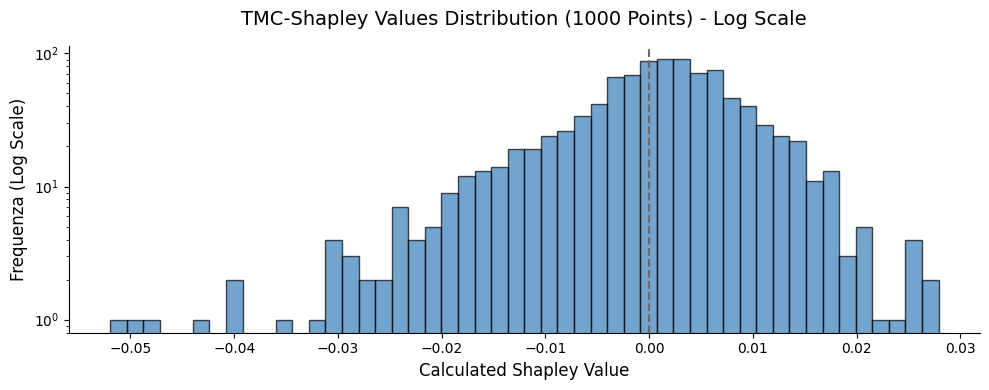
\includegraphics[width=0.9\textwidth]{charts/shapley_distribution_synthetic.png}
    \caption{Data shapley values of the synthetic dataset}
     \label{fig:shapley_distribution_synth}
\end{figure}

The chart \ref{fig:shapley_distribution_bank} shows the distribution of the shapley values for the bank marketing dataset and the chart \ref{fig:shapley_distribution_synth} shows the distribution for the synthetic dataset. 

\begin{table}[h]
\centering
\caption{Top 5 Most and Least Valuable Bank Data Points (Shapley Values)}
\label{tab:rank_bank}
\begin{tabular}{@{}lcc|lcc@{}}
\toprule
\multicolumn{3}{c}{\textbf{Most Valuable}} & \multicolumn{3}{c}{\textbf{Least Valuable}} \\ \cmidrule(lr){1-3} \cmidrule(l){4-6} 
Rank & Index & Shapley Value & Rank & Index & Shapley Value \\ \midrule
1 & 40 & 0.022791 & 1 & 609 & -0.045209 \\
2 & 117 & 0.022571 & 2 & 447 & -0.037279 \\
3 & 176 & 0.017881 & 3 & 381 & -0.028072 \\
4 & 248 & 0.016211 & 4 & 58 & -0.027845 \\
5 & 8 & 0.015610 & 5 & 125 & -0.027730 \\ \bottomrule
\end{tabular}
\end{table}

\begin{table}[h]
\centering
\caption{Top 5 Most and Least Valuable Synthetic Data Points (Shapley Values)}
\label{tab:rank_synth}
\begin{tabular}{@{}lcc|lcc@{}}
\toprule
\multicolumn{3}{c}{\textbf{Most Valuable}} & \multicolumn{3}{c}{\textbf{Least Valuable}} \\ \cmidrule(lr){1-3} \cmidrule(l){4-6} 
Rank & Index & Shapley Value & Rank & Index & Shapley Value \\ \midrule
1 & 718 & 0.027903 & 1 & 516 & -0.051969 \\
2 & 539 & 0.026744 & 2 & 636 & -0.049419 \\
3 & 145 & 0.025864 & 3 & 29 & -0.048023 \\
4 & 120 & 0.025138 & 4 & 857 & -0.042762 \\
5 & 792 & 0.024932 & 5 & 574 & -0.040741 \\ \bottomrule
\end{tabular}
\end{table}

\subsection{Performance vs Fraction removed}
To analyze the quality of the computation, we compared two different approaches, the first one (applied to the bank dataset) by 
fractionally removing $1\%$ of the lowest-value points, that is, each time, after the points are removed, a new model is trained
on the remaining train data, then we calculate the new accuracy.

The second one (with Synthetic dataset) is by fractional removing $1\%$ of the highest-value points.

The chart \ref{fig:fractional_bank} shows how the prediction performance grows faster by fractional removing the worst Shapley values compared with a random removing strategy.

The chart \ref{fig:fractional_synth} shows the reverse strategy for the Synthetic dataset, where the highest values are removed, and as they are removed the performance of the predictor degrades.

\begin{figure}[ht]
    \centering
    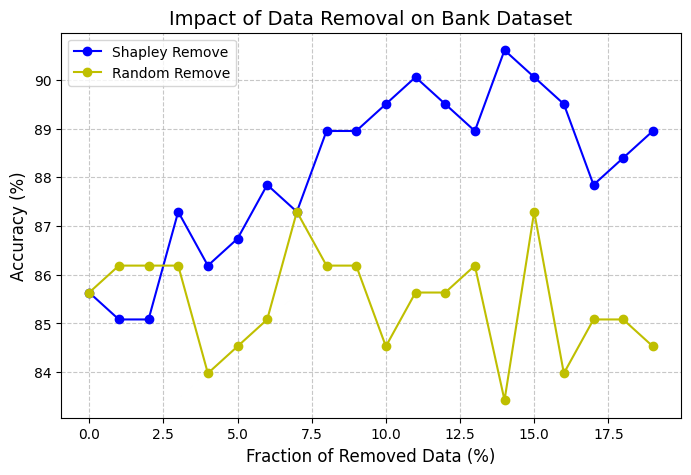
\includegraphics[width=0.9\textwidth]{charts/fractional_remove_bank.png}
    \caption{Fractional Remove(Lowest Value) vs Random Remove for Bank Dataset}
     \label{fig:fractional_bank}
\end{figure}

\begin{figure}[ht]
    \centering
    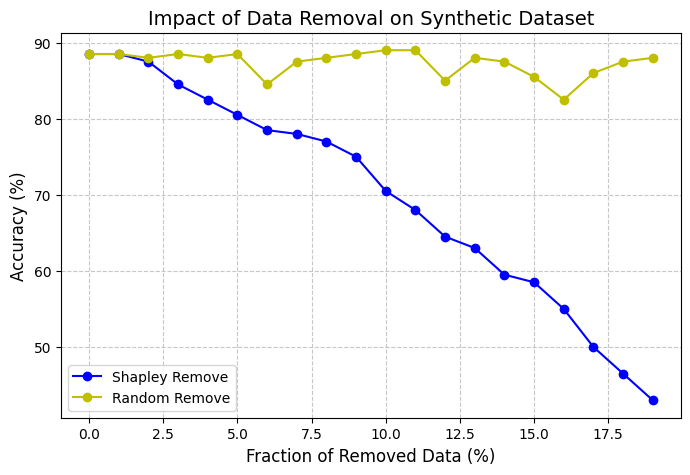
\includegraphics[width=0.9\textwidth]{charts/fractional_remove_synth.png}
    \caption{Fractional Remove(Highest Value) vs Random Remove for Synthetic Dataset}
     \label{fig:fractional_synth}
\end{figure}

\section{Robustness}
To further evaluate the algorithm's robustness in a real-world scenario, we injected label noise into the dataset and analyzed its impact on model accuracy. Furthermore, we inspected training examples ranked from least to most valuable; this confirmed that the algorithm identifies noisy labels significantly faster than a random inspection
\subsection{Inject label noise}
To inject noise we created a method that flips the label (eg. +1 to -1), of our training dataset in a specific percentage (20\%), keeping track of the corrupted indices.
Then we fractionally removed the data points with the lowest Data Shapley values from 0 to 20\%.

In the chart \ref{fig:clean_noisy} we observe that the accuracy grows when removing the lowest values, this shows us that the algorithm, identified the flipped noisy labels correctly.

\begin{figure}[ht]
    \centering
    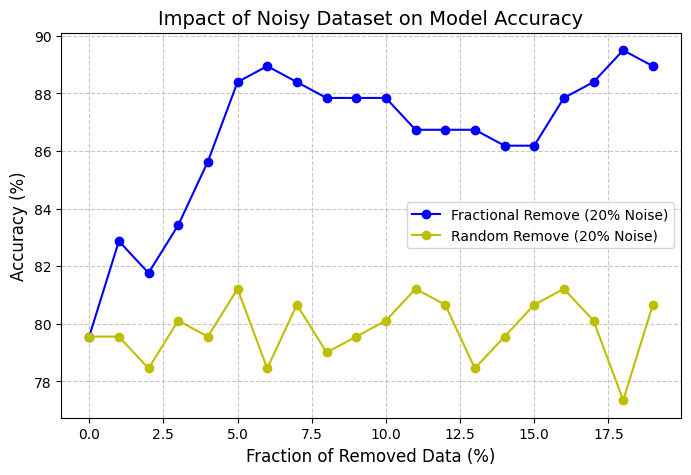
\includegraphics[width=0.9\textwidth]{charts/clean_noisy.png}
    \caption{Flipping labels of Bank Dataset}
     \label{fig:clean_noisy}
\end{figure}


\subsection{Identifying Noisy Data}
In this experiment we flipped 5\% and 10\% of the labels of our training dataset. So we expected that
the flipped labels have the lowest shapley values. Then we calculated the shapley value for these two settings, and 
we started to sequentially inspect our training set from the lowest data shapley value to the highest value to
see if the noisy labels are identified at the beginning, and we compare it with a random inspection.

The chart \ref{fig:mislabel} shows how in both cases (5\% and 10\% noise) 60\% of incorrect labels are identified after an
inspection of less than 20\% of data points, compared with a random inspection that needs a 60\% of inspection. 

\begin{figure}[ht]
    \centering
    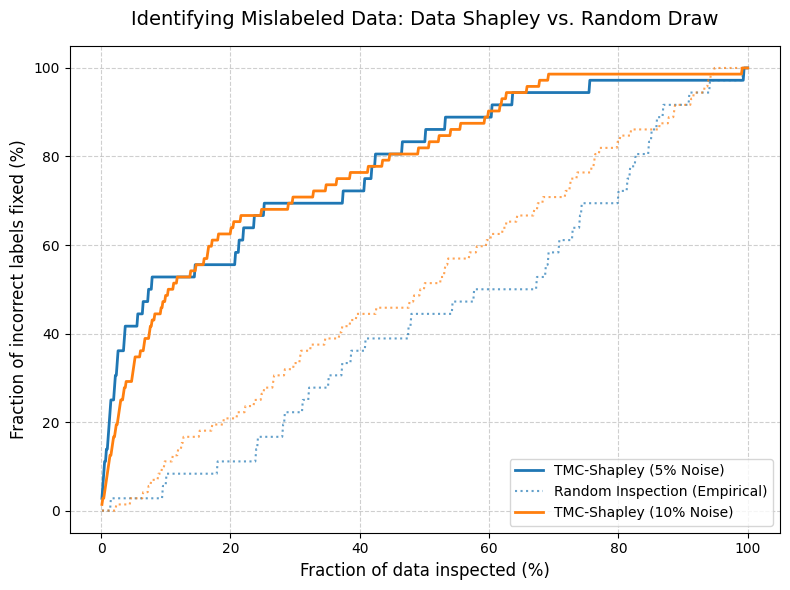
\includegraphics[width=0.9\textwidth]{charts/mislabeled.png}
    \caption{Bank Dataset}
     \label{fig:mislabel}
\end{figure}
\section{Conclusion}
Our evaluations demonstrated that these Shapley values are highly indicative of data quality; sequentially removing the lowest-value data points improved model performance significantly faster than random removal, while discarding high-value points caused rapid performance degradation. 

Furthermore, our robustness experiments confirmed the framework's practical utility in noisy environments. The algorithm efficiently isolated mislabeled data, successfully identifying 60\% of incorrect labels by inspecting less than 20\% of the lowest-ranked data points. 

\section*{Disclaimer}
I declare that this material, which I now submit for assessment, is entirely my own work and has not been taken from the work of others, save and to the extent that such work has been cited and acknowledged within the text of my work. I understand that plagiarism, collusion, and copying are grave and serious offences in the university and accept the penalties that would be imposed should I engage in plagiarism, collusion or copying. This assignment, or any part of it, has not been previously submitted by me or any other person for assessment on this or any other course of study.

\bibliography{references}

\end{document}